% Choose one to switch betweeen slides and handout
%\documentclass[]{beamer}
\documentclass[handout]{beamer}

% Video Meta Data
\title{Smart Contracts and Decentralized Finance}
\subtitle{Account-based Model}
\author{Prof. Dr. Fabian Schär}
\institute{University of Basel}

% Config File
% Packages
\usepackage[utf8]{inputenc}
\usepackage{hyperref}
\usepackage{gitinfo2}
\usepackage{tikz}
 \usetikzlibrary{calc}
\usepackage{amsmath}
\usepackage{mathtools}
\usepackage{bibentry}
\usepackage{xcolor}
\usepackage{colortbl} % Add colour to LaTeX tables
\usepackage{caption}
\usepackage[export]{adjustbox}
\usepackage{pgfplots} \pgfplotsset{compat = 1.17}
\usepackage{makecell}
\usepackage{fancybox}
\usepackage{ragged2e}
\usepackage{fontawesome}
\usepackage{seqsplit}
\usepackage{tabularx}
\usepackage{tcolorbox}
\usepackage{booktabs} % use instead  \hline in tables

% Color Options
\definecolor{highlight}{rgb}{0.65,0.84,0.82}
\definecolor{focus}{rgb}{0.72, 0, 0}
\definecolor{lightred}{rgb}{0.8,0.5,0.5}
\definecolor{midgray}{RGB}{190,195,200}

 %UniBas Main Colors
\definecolor{mint}{RGB}{165,215,210}
\definecolor{anthracite}{RGB}{45,55,60}
\definecolor{red}{RGB}{210,5,55}

 %UniBas Color Palette (for graphics)
\definecolor{strongmint}{RGB}{30,165,165}
\definecolor{darkmint}{RGB}{0,110,110}
\definecolor{softanthracite}{RGB}{140,145,150}
\definecolor{brightanthracite}{RGB}{190,195,200}
\definecolor{softred}{RGB}{235,130,155}

%Custom Colors
\definecolor{lightergray}{RGB}{230, 230, 230}



% Beamer Template Options
\beamertemplatenavigationsymbolsempty
\setbeamertemplate{footline}[frame number]
\setbeamercolor{structure}{fg=black}
\setbeamercolor{footline}{fg=black}
\setbeamercolor{title}{fg=black}
\setbeamercolor{frametitle}{fg=black}
\setbeamercolor{item}{fg=black}
\setbeamercolor{}{fg=black}
\setbeamercolor{bibliography item}{fg=black}
\setbeamercolor*{bibliography entry title}{fg=black}
\setbeamercolor{alerted text}{fg=focus}
\setbeamertemplate{items}[square]
\setbeamertemplate{enumerate items}[default]
\captionsetup[figure]{labelfont={color=black},font={color=black}}
\captionsetup[table]{labelfont={color=black},font={color=black}}

\setbeamertemplate{bibliography item}{\insertbiblabel}

%tcolor boxes
\newtcolorbox{samplecode}[2][]{
  colback=mint, colframe=darkmint, coltitle=white,
  fontupper = \ttfamily\scriptsize, fonttitle= \bfseries\scriptsize,
  boxrule = 0mm, arc = 0mm,
  boxsep = 1.3mm, left = 0mm, right = 0mm, top = 0.5mm, bottom = 0mm, middle=0mm,
  #1,title=#2}
  
\newtcolorbox{keytakeaway}[2][]{
  colback=softred, colframe=red, coltitle=white,
  fontupper = \scriptsize, fonttitle= \bfseries\scriptsize,
  boxrule = 0mm, arc = 0mm,
  boxsep = 1.3mm, left = 0mm, right = 0mm, top = 0.5mm, bottom = 0mm, middle=0mm,
  #1,title=#2}

\newtcolorbox{exercise}[2][]{
  colback=brightanthracite, colframe=anthracite, coltitle=white,
  fontupper = \scriptsize, fonttitle= \bfseries\scriptsize,
  boxrule = 0mm, arc = 0mm,
  boxsep = 1.3mm, left = 0mm, right = 0mm, top = 0.5mm, bottom = 0mm, middle=0mm,
  #1,title=#2}



% Link Icon Command 
\newcommand{\link}{%
    \tikz[x=1.2ex, y=1.2ex, baseline=-0.05ex]{%
        \begin{scope}[x=1ex, y=1ex]
            \clip (-0.1,-0.1)
                --++ (-0, 1.2)
                --++ (0.6, 0)
                --++ (0, -0.6)
                --++ (0.6, 0)
                --++ (0, -1);
            \path[draw,
                line width = 0.5,
                rounded corners=0.5]
                (0,0) rectangle (1,1);
        \end{scope}
        \path[draw, line width = 0.5] (0.5, 0.5)
            -- (1, 1);
        \path[draw, line width = 0.5] (0.6, 1)
            -- (1, 1) -- (1, 0.6);
        }
    }

% Other commands
\newcommand\tab[1][0.5cm]{\hspace*{#1}} % for code boxes


% Read Git Data from Github Actions Workflow
% Defaults to gitinfo2 for local builds
\IfFileExists{gitInfo.txt}
	{\input{gitInfo.txt}}
	{
		\newcommand{\gitRelease}{(Local Release)}
		\newcommand{\gitSHA}{\gitHash}
		\newcommand{\gitDate}{\gitAuthorIsoDate}
	}

% Custom Titlepage
\defbeamertemplate*{title page}{customized}[1][]
{
  \vspace{-0cm}\hfill\includegraphics[width=2.5cm]{../config/logo_cif}
  \includegraphics[width=1.9cm]{../config/seal_wwz}
  \\ \vspace{2em}
  \usebeamerfont{title}\textbf{\inserttitle}\par
  \usebeamerfont{title}\usebeamercolor[fg]{title}\insertsubtitle\par  \vspace{1.5em}
  \small\usebeamerfont{author}\insertauthor\par
  \usebeamerfont{author}\insertinstitute\par \vspace{2em}
  \usebeamercolor[fg]{titlegraphic}\inserttitlegraphic
    \tiny \noindent \texttt{Release Ver.: \gitRelease}\\ 
    \texttt{Version Hash: \gitSHA}\\
    \texttt{Version Date: \gitDate}\\ \vspace{1em}
    
    
    \iffalse
  \link \href{https://github.com/cifunibas/Bitcoin-Blockchain-Cryptoassets/blob/main/slides/intro.pdf}
  {Get most recent version}\\
  \link \href{https://github.com/cifunibas/Bitcoin-Blockchain-Cryptoassets/blob/main/slides/intro.pdf}
  {Watch video lecture}\\ 
  
  \fi
  
  \vspace{1em}
  License: \texttt{Creative Commons Attribution-NonCommercial-ShareAlike 4.0 International}\\\vspace{2em}
  \includegraphics[width = 1.2cm]{../config/license}
}


% tikzlibraries
\usetikzlibrary{decorations.pathreplacing}
\usetikzlibrary{decorations.markings}
\usetikzlibrary{positioning}
\usetikzlibrary{calc}
\captionsetup{font=footnotesize}

%%%%%%%%%%%%%%%%%%%%%%%%%%%%%%%%%%%%%%%%%%%%%%
%%%%%%%%%%%%%%%%%%%%%%%%%%%%%%%%%%%%%%%%%%%%%%
\begin{document}

\thispagestyle{empty}
\begin{frame}[noframenumbering]
	\titlepage
\end{frame}


%%%
\begin{frame}{Programmable Money Paradigms}
	\begin{columns}[T]
		\begin{column}{0.45\textwidth}
			\centering
			\includegraphics[scale=0.075]{../assets/images/bitcoin_network_symbol.png}\\
			\textbf{UTXO Model}
		\end{column}
		\begin{column}{0.45\textwidth}
			\centering
			\includegraphics[scale=0.1]{../assets/images/EOA.png}
			\includegraphics[scale=0.1]{../assets/images/CA.png}
			\textbf{Account-based Model}
		\end{column}
	\end{columns}
	\vspace{1em}
	\begin{columns}[T]
		\begin{column}{0.45\textwidth}
		\vspace{1em}
			\begin{itemize}
				\item Conditions are on each UTXO.
				\item Determine how this UTXO can be spend.
			\end{itemize}
		\end{column}
		\begin{column}{0.45\textwidth}
		\vspace{1em}
			\begin{itemize}
				\item Conditions are on each account.
				\item Determine how the account is governed.
			\end{itemize}
		\end{column}
	\end{columns}
\vspace{1em}
\uncover<2->{
	\begin{keytakeaway}{Key Takeaway}
		The ability to implement logic on an account level allows for all sorts of use-cases. It is more flexible, more intuitive and easier to handle than conditions on the UTXO-level.
	\end{keytakeaway}
	}
\end{frame}
%%%


%%%
\begin{frame}{Accounts}
Instead of Bitcoin's UTXO model, Ethereum uses actual accounts.
	\vspace{1em}
		\begin{itemize}
			\item<1-> Each account has a 20 byte address.
			\item<1-> Hexadecimal encoding
		\end{itemize}
	\vspace{1em}
	Example: \texttt{OxD3EEC7A7C7867B9D02248B414F08609A2A6C2AB4}
\end{frame}
%%%	


%%%
\begin{frame}{EIP-55: Capital letter checksum}
No checksum encoding $\rightarrow$ Typos were a severe problem. \\ 
\vspace{2em}
	\textbf{\link \href{https://eips.ethereum.org/EIPS/eip-55}{EIP-55}} fixes this: Use keccak hash function $H(x)=h$, where input $x$ corresponds to the address and $h$ to the hash value. For each character (a-f) at position $x[i]$, capitalize $x[i]$, if $h[i] > 7$.\\
\vspace{2em}
\uncover<2->{
	\texttt{Keccak(0xD3EEC7A7C7867B9D02248B414F08609A2A6C2AB4)} = \\
\vspace{0.5em}

	\hspace{4.75em}\texttt{\textcolor{highlight}{e}1\textcolor{focus}{254}6\textcolor{focus}{7}9\textcolor{highlight}{f}8029\textcolor{highlight}{e}f\textcolor{focus}{7}c379d\textcolor{focus}{6}0b9\textcolor{highlight}{a}49f44\textcolor{highlight}{8}9\textcolor{highlight}{f}b\textcolor{focus}{4}c\textcolor{highlight}{8}\textcolor{focus}{7}2\dots}  \\
	  
\vspace{0.5em}

	\hspace{3.7em}\texttt{0xD3\textcolor{focus}{eec}7\textcolor{focus}{a}7\textcolor{highlight}{C}7867\textcolor{highlight}{B}9\textcolor{focus}{d}02248\textcolor{focus}{b}414\textcolor{highlight}{F}08609\textcolor{highlight}{A}2\textcolor{highlight}{A}6\textcolor{focus}{c}2\textcolor{highlight}{A}\textcolor{focus}{b}4}
	}
\end{frame}
%%%


%%%
\begin{frame}{Different Types of Accounts}

	\begin{columns}[T]
		\begin{column}{0.45\textwidth}
			\centering
			\includegraphics[scale=0.09]{../assets/images/EOA.png} \\
			\textbf{Externally Owned Accounts}
		\end{column}
		\begin{column}{0.45\textwidth}
		\centering
			\includegraphics[scale=0.093]{../assets/images/CA.png}\\
			\textbf{Contract Accounts}
		\end{column}
	\end{columns}  
\vspace{1em}
	\begin{columns}[T]
		\begin{column}{0.45\textwidth}
			\begin{itemize}
				\item Address
				\item Balance
				\item Nonce (\# of transactions)
			\end{itemize}
		\end{column}
		\begin{column}{0.45\textwidth}
			\begin{itemize}
				\item Address
				\item Balance
				\item Nonce (\# of accounts created)
				\item Contract code
				\item Contract storage
			\end{itemize}
		\end{column}
	\end{columns}
\vspace{1em}
\uncover<2->{
	\begin{keytakeaway}{Control Over Accounts}
		 Externally  Owned  Accounts  are  controlled  by  a  private  key.  Contract accounts are controlled by the contract code.
	\end{keytakeaway}	
	}			
\end{frame}
%%%


%%%
\begin{frame}{How Contract Accounts are created}

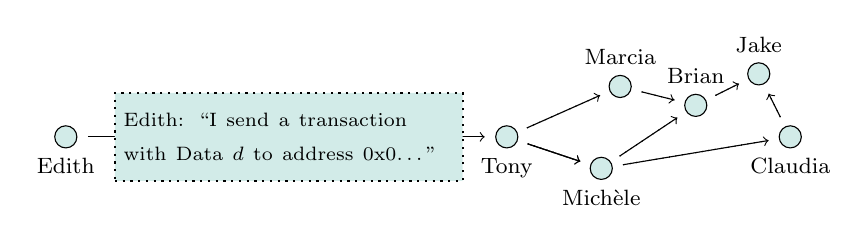
\begin{tikzpicture}[domain=-8:8, scale=0.8]

% transaction
	\coordinate (c1) at (0,0);
	\coordinate (c2) at (7,0);
	\filldraw[draw=black,fill=highlight!50] (c1) circle (5pt) node[below=0.15cm,color=black]{\footnotesize{Edith}};
	\draw[shorten >=0.28cm,shorten <=0.28cm,->] (c1) to[] (c2);

% network

\coordinate (c3) at (8.8,0.8);
\coordinate (c4) at (8.5,-0.5);
\coordinate (c5) at (10,0.5);
\coordinate (c6) at (11,1);
\coordinate (c7) at (11.5,0);
\filldraw[draw=black,fill=highlight!50] (c2) circle (5pt) node[below=0.15cm,color=black]{\footnotesize{Tony}};
\filldraw[draw=black,fill=highlight!50] (c3) circle (5pt) node[above=0.15cm,color=black]{\footnotesize{Marcia}};
\filldraw[draw=black,fill=highlight!50] (c4) circle (5pt) node[below=0.15cm,color=black]{\footnotesize{Michèle}};
\filldraw[draw=black,fill=highlight!50] (c5) circle (5pt) node[above=0.15cm,color=black]{\footnotesize{Brian}};
\filldraw[draw=black,fill=highlight!50] (c6) circle (5pt) node[above=0.15cm,color=black]{\footnotesize{Jake}};
\filldraw[draw=black,fill=highlight!50] (c7) circle (5pt) node[below=0.15cm,color=black]{\footnotesize{Claudia}};


\draw[shorten >=0.28cm,shorten <=0.28cm,->] (c2) to[] (c3);
\draw[shorten >=0.28cm,shorten <=0.28cm,->] (c2) to[] (c4);
\draw[shorten >=0.28cm,shorten <=0.28cm,->] (c2) to[] (c4);
\draw[shorten >=0.28cm,shorten <=0.28cm,->] (c3) to[] (c5);
\draw[shorten >=0.28cm,shorten <=0.28cm,->] (c4) to[] (c5);
\draw[shorten >=0.28cm,shorten <=0.28cm,->] (c4) to[] (c7);
\draw[shorten >=0.28cm,shorten <=0.28cm,->] (c5) to[] (c6);
\draw[shorten >=0.28cm,shorten <=0.28cm,->] (c7) to[] (c6);


\draw[shorten >=0.28cm,shorten <=0.28cm, dotted] (c2) to[] (c3);
\draw[shorten >=0.28cm,shorten <=0.28cm, dotted] (c2) to[] (c4);
\draw[shorten >=0.28cm,shorten <=0.28cm, dotted] (c2) to[] (c4);
\draw[shorten >=0.28cm,shorten <=0.28cm, dotted] (c3) to[] (c5);
\draw[shorten >=0.28cm,shorten <=0.28cm, dotted] (c4) to[] (c5);
\draw[shorten >=0.28cm,shorten <=0.28cm, dotted] (c4) to[] (c7);
\draw[shorten >=0.28cm,shorten <=0.28cm, dotted] (c5) to[] (c6);
\draw[shorten >=0.28cm,shorten <=0.28cm, dotted] (c7) to[] (c6);


% smart contract deployment

\filldraw[fill=highlight!50,dotted,thick] (0.78,-0.7) -- (6.3,-0.7) -- (6.3,0.7) -- (0.78,0.7) -- (0.78,-0.7) node[midway, right=-0.02cm,text width=4.25cm]{\scriptsize{Edith: ``I send a transaction with Data $d$ to  address 0x0\dots ''}};



\end{tikzpicture}

\begin{enumerate}
				\item<1-> EOA or CA issues transaction with \textbf{zero address} as recipient address.
				\vspace{1em}
				\item<2-> The transaction carries the contract code.
				\item<3-> Transaction confirmation = Contract deployment
				\item<4-> New Contract Account address = \texttt{SHA3.256(address\_sender, nonce)} %corresponds to hash value of the deployment transaction sender's address and the transaction nonce.
\end{enumerate}
			
\end{frame}
%%%	


%%%
\begin{frame}{Contract Account Code and ABI}
	\begin{columns}[T]
		\begin{column}{0.6\textwidth}
			\begin{figure}[h!]
				\center
					\begin{tikzpicture}[scale=0.9]

\draw(-4.5,-2) node[right] {\includegraphics[scale=0.5]{../assets/images/solidity_code.png}} node[below] at (-3.3, -3.2) {Solidity Code} node[below] at (-3.3, -3.7) {{\tiny Vyper}} node[below] at (-3.3, -4) {{\tiny LLL(Lower-Level Lisp-like Language)}};

\draw [decorate,decoration={brace,amplitude=5pt,mirror},xshift=4pt,yshift=0pt]
    (-1.3,0) -- (-1.3,-4.6) node[right, rotate=90] at (-1,-3.2)  
    {\footnotesize compiles to};

\draw(-0.4,-0.4) node[right] {\includegraphics[scale=0.1]{../assets/images/binary_code.png}};

\draw(-0.2,-4) node[right] {\includegraphics[scale=0.5]{../assets/images/ABI.png}};

\end{tikzpicture}
			\end{figure}\vspace{1em}
		\end{column}
		\begin{column}{0.5\textwidth}
			\textbf{Bytecode}
				\begin{itemize}
					\item Deployed on Blockchain
					\item Actual Code that gets executed
				\end{itemize}
		\vspace{2em}
			\textbf{Application Binary Interface}
				\begin{itemize}
					\item List of contract functions and their arguments (JSON)
					\item En- \& Decoding of Data (Translation) 
				\end{itemize}
		\end{column}
	\end{columns}
\vspace{1em}
	\begin{keytakeaway}{The ABI is needed for User Interaction}
		 Without the ABI, applications would not know the available functions and function arguments. The ABI can be seen as a translation or contract specification.
	\end{keytakeaway}		
\end{frame}
%%%


%%%
\begin{frame}{Account-based Model vs. UTXO-based Model}
	The account based model may be more intuitive at first, however, it does have some drawbacks compared to the UTXO model. \\ 
	\vspace{2em}
		\begin{columns}[T]
			\begin{column}{0.25\textwidth}
				\center
				\includegraphics[scale=0.1]{../assets/images/privacy.png}
			\end{column}
			\begin{column}{0.8\textwidth}
				\textbf{Privacy Concerns}\\
People usually use the same address for many transactions - in contrast to UTXO based systems where you use a new address for each transaction. \\
\href{https://etherscan.io/address/0x8cbcb10a365a5e26dfcd41b1257fda54bc604c70}{\link {\small Etherscan}}
			\end{column}
		\end{columns}	
\end{frame}
%%%


%%%
\begin{frame}{Account-based vs. UTXO-based Model}
	\begin{columns}[T]
		\begin{column}{0.25\textwidth}
			\center
			\includegraphics[scale=0.1]{../assets/images/alert.png}
		\end{column}
		\begin{column}{0.8\textwidth}
			\textbf{Transactions getting stuck}\\
			If a transaction from an account has not been confirmed yet, subsequent ones from the same account won't get through.
		\end{column}
	\end{columns}
	\vspace{2em}
\uncover<2->{
	\begin{columns}[T]
		\begin{column}{0.25\textwidth}
			\center
			\includegraphics[scale=0.1]{../assets/images/argument.png}
		\end{column}
		\begin{column}{0.8\textwidth}
			\textbf{Unintended Conflicts}\\
If two wallet applications are not in sync, two transactions A and B may be conflicting, even if the total balance of the account is larger than the aggregated amount sent with transactions A and B (same Problem with SC).
		\end{column}
	\end{columns}
		}
\end{frame}
%%%


%%%
\begin{frame}{Creating and Funding A Metamask Account}

	\begin{exercise}{Exercise 1:}
		\begin{enumerate}
			\item Get the Metamask Browser extension (available for Chrome, Firefox and Brave)
			\item Set up a new account and make sure you are connected to Ropsten testnet.
			\item Backup the mnemonic phrase of your wallet.
			\item Go to \link \href{https://faucet.metamask.io/}{Test Ether Faucet} and get some Ropsten Ether.
		\end{enumerate}
	\end{exercise}	
\uncover<2->{		
	\begin{columns}[T]
		\begin{column}{0.2\textwidth}
			\center
			\includegraphics[scale=0.1]{../assets/images/alert.png}
		\end{column}
		\begin{column}{0.8\textwidth}
		\vspace{1em}
		If you are currently managing Mainnet funds with Metamask, make sure \textcolor{focus}{NOT} to use the same mnemonic seed for your testnet transactions. In doing so you will put your ETH and tokens at risk.
		\end{column}
	\end{columns}
}
\end{frame}
%%%	


%%%
\begin{frame}{Creating and Funding A Metamask Account}

	\begin{exercise}{Exercise 2:}
		\begin{enumerate}
			\item Enter your address on the \link ???
			\item Transfer 0.1 Ropsten ETH to the address in the row below your own address.
			\item Check the transaction details on \link \href{https://ropsten.etherscan.io/}{Ropsten Etherscan}
		\end{enumerate}
	\end{exercise}	
\end{frame}
%%%	

\end{document}